\documentclass[12pt,a4paper,oneside]{article}
\usepackage{amsmath,amssymb}
\usepackage{fancyhdr}
\usepackage{enumerate}
\usepackage{tkz-euclide}
%\usetkzobj{all}
\usepackage{tikz-3dplot}
%\usetikzlibrary{arrows}
\usetikzlibrary{shapes.geometric}
\usepackage{wasysym}
\usepackage[tikz]{bclogo}
\usetkzobj{all}
\usepackage{tikz,tkz-tab,tkz-linknodes}
\usetikzlibrary{snakes}
\usepackage{tabvar}
 
\usepackage{pgfplots}
\usepgfplotslibrary{fillbetween}
\usetikzlibrary{patterns}
\pgfplotsset{compat=1.9}

\usetikzlibrary{arrows,calc,intersections,angles}
\usepackage[top=2cm, bottom=2cm, left=2cm, right=1.5cm] {geometry}
%\usepackage[unicode, bookmarks=false]{hyperref}
\usepackage[hidelinks,unicode]{hyperref}

\usepackage{currfile}

\usepackage[loigiai]{ex_test} 
%\usepackage[loigiai]{ex_test}
%\usepackage[color]{ex_test}
%\renewtheorem{ex}{\color{violet}Câu}
\newtheorem{vd}{Ví dụ}
\newtheorem{bt}{Bài}
\newtheorem{dn}{Định nghĩa}
\usepackage{esvect}
\def\vec{\vv}
\def\overrightarrow{\vv}
%Lệnh của gói mathrsfs
\DeclareSymbolFont{rsfs}{U}{rsfs}{m}{n}
\DeclareSymbolFontAlphabet{\mathscr}{rsfs}
%Lệnh cung
\DeclareSymbolFont{largesymbols}{OMX}{yhex}{m}{n}
\DeclareMathAccent{\wideparen}{\mathord}{largesymbols}{"F3}
%Lệnh song song
\DeclareSymbolFont{symbolsC}{U}{txsyc}{m}{n}
\DeclareMathSymbol{\varparallel}{\mathrel}{symbolsC}{9}
\DeclareMathSymbol{\parallel}{\mathrel}{symbolsC}{9}
%Hệ hoặc, hệ và
\newcommand{\hoac}[1]{ 
\left[\begin{aligned}#1\end{aligned}\right.}
\newcommand{\heva}[1]{
\left\{\begin{aligned}#1\end{aligned}\right.}
\renewcommand{\baselinestretch}{1.5}
\hidetextchoice
\begin{document}

\Opensolutionfile{ans}[ans/anstest]
\Opensolutionfile{ansshort}[ans/ansshort1]
	\title{Một số tính năng của  \texttt{ex\_test} bản 2.4.3}
	\author{Trần Anh Tuấn, Đại học Thương Mại}
	\maketitle
%	\tableofcontents
%	\newpage
% Môi trường liệt kê dàn theo nhiều dòng khác nhau
\section{Môi trường liệt kê chia cột}
\subsection{Lệnh listEX}
\subsubsection{Cấu trúc}
\begin{verbatim}
\begin{listEX}[Số cột]%Bỏ trống tùy chọn số cột thì sẽ trở thành 1 cột
\item 
\item 
\end{listEX}
\end{verbatim}
\begin{ex}
Giải các phương trình sau
\begin{listEX}[3]
\item $x^2-x+1=0$;
\item $x^2+1=0$;
\item $x^2-1=0$;
\item $x^2+x-1=0$;
\item $x^2-3x+2=0$;
\end{listEX}
\end{ex}
\begin{ex}
Các khẳng định sau là đúng hay sai?
\begin{listEX}
	\item Cho $a$, $b$ là hai đường thẳng chéo nhau và vuông góc với nhau. Đường vuông góc chung của $a$ và $b$ nằm trong mặt phẳng chứa đường này và vuông góc với đường kia. 
	\item Không thể có một hình chóp tứ giác $S.ABCD$ nào có hai mặt bên $(SAB)$ và $(SCD)$ cùng vuông góc với mặt đáy.
	\item Cho $\vec{u}$, $\vec{v}$ là hai véc-tơ chỉ phương của hai đường thẳng cắt nhau nằm trong mặt phẳng $(\alpha)$ và $\vec{n}$ là véc-tơ chỉ phương của đường thẳng $\Delta$. Điều kiện cần và đủ để $\Delta\perp(\alpha)$ là $\vec{n}\cdot\vec{u}=0$ và $\vec{n}\cdot\vec{v}=0$.
	\item Hai đường thẳng $a$ và $b$ trong không gian có các véc-tơ chỉ phương lần lượt là $\vec{u}$ và $\vec{v}$. Điều kiện cần và đủ để $a$ và $b$ chéo nhau là $a$ và $b$ không có điểm chung và hai véc-tơ $\vec{u}$ và $\vec{v}$ không cùng phương.
\end{listEX}
\end{ex}
\subsubsection{Thay bộ đếm môi trường list}
\begin{verbatim}
\def\listEXenumi{Nội dung thay đổi bộ đếm của enumi hoặc kí tự bất kì}
\end{verbatim}
\begin{center}
\begin{tabular}{|l|l|}
\hline 
 \verb+\def\listEXenumi{\alph{enumi})}+&Kiểu chữ cái thường a), b),... (mặc định) \\ 
\hline 
 \verb+\def\listEXenumi{\Alph{enumi})}+ & Chữ cái in hoa A), B),...\\ 
\hline 
 \verb+\def\listEXenumi{\arabic{enumi}.}+ & Đánh số 1., 2.,... \\ 
\hline 
 \verb+\def\listEXenumi{(\roman{enumi})}+ & Chữ số La Mã thường (i), (ii),... \\ 
\hline 
 \verb+\def\listEXenumi{(\roman{enumi})}+ & Chữ số La Mã in hoa (I), (II),... \\ 
\hline 
 \verb+\def\listEXenumi{{\color{red}$\square$}}+ & Kí tự đặc biệt: ô vuông màu đỏ,... \\ 
\hline 
\end{tabular} 
\end{center}
\def\listEXenumi{(\roman{enumi})}
\begin{ex}
Giải các phương trình sau
\begin{listEX}[3]
\item $x^2-x+1=0$;
\item $x^2+1=0$;
\item $x^2-1=0$;
\item $x^2-x-1=0$;
\item $x^2+x-1=0$;
\item $x^2-3x-1=0$;
\end{listEX}
\end{ex}
\def\listEXenumi{{\color{red}\checked}}
\begin{ex}
Giải các phương trình sau
\begin{listEX}[3]
\item $x^2-x+1=0$;
\item $x^2+1=0$;
\item $x^2-1=0$;
\item $x^2-x-1=0$;
\item $x^2+x-1=0$;
\item $x^2-3x-1=0$;
\end{listEX}
\end{ex}
\def\listEXenumi{{\color{red}$\square$}}
\begin{ex}
Giải các phương trình sau
\begin{listEX}[3]
\item $x^2-x+1=0$;
\item $x^2+1=0$;
\item $x^2-1=0$;
\item $x^2-x-1=0$;
\item $x^2+x-1=0$;
\item $x^2-3x-1=0$;
\end{listEX}
\end{ex}
\subsubsection{Thay đổi số thứ tự  liệt đầu tiên}
\begin{verbatim}
\setcounter{enumi}{n-1}%n là số thứ tự liệt kê đầu tiên
\end{verbatim}
\def\listEXenumi{\alph{enumi})}
Chẳng hạn, muốn thứ tự liệt kê đầu tiên là d) (số thứ tự n=4 trong bảng chữ cái)
\setcounter{enumi}{3}
\begin{ex}
Giải các phương trình sau
\begin{listEX}[3]
\item $x^2-x+1=0$;
\item $x^2+1=0$;
\item $x^2-1=0$;
\item $x^2-x-1=0$;
\item $x^2+x-1=0$;
\item $x^2-3x-1=0$;
\end{listEX}
\end{ex}
\subsection{Lệnh enumEX}
\subsubsection{Cấu trúc tổng quát}
\begin{verbatim}
\begin{enumEX}[Kiểu liệt kê: a), (1), i.,...]{Số cột}
\item 
\item 
\end{enumEX}
\end{verbatim}
\begin{ex}
Giải các phương trình sau
\begin{enumEX}[(i)]{3}
\item $x^2-x+1=0$;
\item $x^2+1=0$;
\item $x^2-1=0$;
\item $x^2+x-1=0$;
\item $x^2-3x+2=0$;
\end{enumEX}
\end{ex}
\begin{ex}
Giải các phương trình sau
\begin{enumEX}[(a)]{3}
\item $\dfrac{x^2+1}{x+1}=0$;
\item $x^2-x+1=0$;
\item $x^2-1=0$;
\item $x^2+x-1=0$;
\item $\dfrac{x^2-x-1}{x-1}=0$;
\end{enumEX}
\end{ex}
\subsubsection{Cấu trúc rút gọn}
Nếu tùy chọn kiểu liệt kê bỏ qua thì kiểu liệt kê mặc định là a)
\begin{verbatim}
\begin{enumEX}{Số cột}
\item 
\item 
\end{enumEX}
\end{verbatim}
\begin{ex}
Các khẳng định sau là đúng hay sai?
\begin{enumEX}{1}
	\item\TF{Đ} Cho $a$, $b$ là hai đường thẳng chéo nhau và vuông góc với nhau. Đường vuông góc chung của $a$ và $b$ nằm trong mặt phẳng chứa đường này và vuông góc với đường kia. 
	\item\TF{S}  Không thể có một hình chóp tứ giác $S.ABCD$ nào có hai mặt bên $(SAB)$ và $(SCD)$ cùng vuông góc với mặt đáy.
	\item\TF{S}   Cho $\vec{u}$, $\vec{v}$ là hai véc-tơ chỉ phương của hai đường thẳng cắt nhau nằm trong mặt phẳng $(\alpha)$ và $\vec{n}$ là véc-tơ chỉ phương của đường thẳng $\Delta$. Điều kiện cần và đủ để $\Delta\perp(\alpha)$ là $\vec{n}\cdot\vec{u}=0$ và $\vec{n}\cdot\vec{v}=0$.
	\item\TF{S}  Hai đường thẳng $a$ và $b$ trong không gian có các véc-tơ chỉ phương lần lượt là $\vec{u}$ và $\vec{v}$. Điều kiện cần và đủ để $a$ và $b$ chéo nhau là $a$ và $b$ không có điểm chung và hai véc-tơ $\vec{u}$ và $\vec{v}$ không cùng phương.
\end{enumEX}
\end{ex}
\subsubsection{Thay đổi số thứ tự  liệt đầu tiên}
\begin{verbatim}
\begin{enumEX}[]{}\setcounter{enumi}{n-1}%n là số thứ tự liệt kê đầu tiên
\end{verbatim}
\begin{ex}
Giải các phương trình sau
\begin{enumEX}{3}\setcounter{enumi}{3}
\item $\dfrac{x^2+1}{x+1}=0$;
\item $x^2-x+1=0$;
\item $x^2-1=0$;
\item $x^2+x-1=0$;
\item $\dfrac{x^2-x-1}{x-1}=0$;
\end{enumEX}
\end{ex}
\subsubsection{Vấn đề dãn dòng khi số cột lớn hơn 1}
enumEX bị hạn chế là dãn dòng theo chiều cao của 2 \verb+\item+ đầu tiên của mỗi dòng, vì vậy trong một số trường hợp việc dãn dàng không được như mong đợi, chẳng hạn
\begin{ex}
Giải các phương trình sau
\begin{enumEX}{3}
\item $x^2-x+1=0$;
\item $\color{violet}\dfrac{x^2+1}{x+1}=0$;
\item $x^2-1=0$;
\item $x^2+x-1=0$;
\item $\color{violet}\dfrac{x^2-x-1}{x-1}=0$.
\end{enumEX}
\end{ex}
\textbf{Một số cách khắc phục tạm thời khi chờ các cập nhật sau}\\
\textbf{\textit{Cách 1:}} Chuyển sang dùng môi trường listEX
\begin{ex}
Giải các phương trình sau
\begin{listEX}[3]
\item $x^2-x+1=0$;
\item $\dfrac{x^2+1}{x+1}=0$;
\item $x^2-1=0$;
\item $x^2+x-1=0$;
\item $\dfrac{x^2-x-1}{x-1}=0$.
\end{listEX}
\end{ex}
\textbf{\textit{Cách 2:}} Thay đổi thứ tự các \verb+\item+ nếu có thể
\begin{ex}
Giải các phương trình sau
\begin{enumEX}{3}
\item $\dfrac{x^2+1}{x+1}=0$;
\item $x^2-x+1=0$;
\item $x^2-1=0$;
\item $x^2+x-1=0$;
\item $\dfrac{x^2-x-1}{x-1}=0$;
\end{enumEX}
\end{ex}
\textbf{\textit{Cách 3:}} Thêm khoảng lệnh khoảng cách giữa hai dòng (chẳng hạn \verb+\vspace{8pt}+)
\begin{ex}
Giải các phương trình sau
\begin{enumEX}{3}
\item $x^2-x+1=0$;
\item $\dfrac{x^2+1}{x+1}=0$;
\item $x^2-1=0$;\vspace{8pt}
\item $x^2+x-1=0$;
\item $\dfrac{x^2-x-1}{x-1}=0$.
\end{enumEX}
\end{ex}

\section{Ẩn hiện văn bản trong \LaTeX}
\subsection{Tổng quát}
\begin{verbatim}
\sh{NỘI DUNG}%\sh viết tắt của \showhide
\end{verbatim}

Khi bật tùy chọn loigiai hoặc solcolor thì \textbf{NỘI DUNG} sẽ được hiển thị. Nếu bật tùy chọn dethi thì \textbf{NỘI DUNG} sẽ bị ẩn, thay vào đó sẽ là một đường kẻ ngang có độ dài bằng độ dài của \textbf{NỘI DUNG} và để thừa một hộp văn bản trống đúng bằng \textbf{NỘI DUNG}.
\begin{ex}
	Thể tích khối chóp được tính bởi công thức \sh{$V=\dfrac{1}{3}S.h$}, trong đó $S$ là diện tích đáy và $h$ là đường cao của khối chóp.
\end{ex}
\begin{ex}
	Cho tứ diện gần đều $ABCD$ với $AB=CD=a$, $AC~=~BD~=~b$, $AD=BC=c$ có thể tích được tính bởi \sh{$V=\dfrac{1}{6\sqrt{2}}\sqrt{(-a^2+b^2+c^2)(a^2-b^2+c^2)(a^2+b^2-c^2)}$}.
\end{ex}
\begin{ex}
	Công thức thể tích tứ diện $S.ABC$ là \sh{$V=\dfrac{1}{12\sqrt{2}}\sqrt{
	\left|\begin{array}{ccc}
	2a^2&a^2+b^2-z^2&a^2+c^2-y^2\\
	a^2+b^2-z^2&2b^2&b^2+c^2-x^2\\
	a^2+c^2-y^2&b^2+c^2-x^2&2c^2
	\end{array}\right|
	}$}, trong đó $SA=a$, $SB=b$, $SC=c$, $BC=x$, $CA=y$, $AB=z$.
\end{ex}

\begin{ex}
	Cho tam giác $ABC$ vuông tại $A$. Định lí Pytago phát biểu là \sh{$a^2=b^2+c^2$}, trong đó  $BC=a$, $CA=b$, $AB=c$. 
\end{ex}
\subsection{Lệnh \texttt{boxEX}}
\begin{verbatim}
\boxEX{NỘI DUNG}
\end{verbatim}
Hoặc để thay đổi kích thước hộp thì dùng lệnh
\begin{verbatim}
\boxEX[kích thước]{NỘI DUNG}
\end{verbatim}
Khi bật tùy chọn loigiai hoặc solcolor thì sẽ hiển thị  \textbf{NỘI DUNG}, chẳng hạn \boxEX{$\in$}. \\
Nếu bật tùy chọn dethi thì \textbf{NỘI DUNG} sẽ bị ẩn, thay vào đó sẽ hiện một ô vuông trống \boxEX{}
\begin{ex}
	Điền kí hiệu $\in, \not\in, \subset$ thích hợp vào ô vuông:
	\begin{listEX}[3]
		\item $-3\boxEX{$\not\in$}\mathbb{N}$;
		\item $\dfrac{2}{3}\boxEX{$\in$}\mathbb{Q}$;
		\item $\mathbb{Z}\boxEX[0.7cm]{$\subset$}\mathbb{Q}$.
	\end{listEX}
\end{ex}
\subsection{Lệnh \texttt{TF}}
\begin{verbatim}
\TF{NỘI DUNG}%\TF viết tắt của TrueFalse
\end{verbatim}
Khi bật tùy chọn loigiai hoặc solcolor thì sẽ hiển thị  \textbf{NỘI DUNG}, chẳng hạn \TF{Đ}. \\
Nếu bật tùy chọn dethi thì \textbf{NỘI DUNG} sẽ bị ẩn, thay vào đó sẽ hiện một ô vuông trống \boxEX{}
\begin{ex}
	Các khẳng định sau là đúng hay sai?
	\begin{enumerate}
		\item \TF{Đ} $\sqrt{2}$ là số vô tỉ;
		\item \TF{S} $3>5$;
		\item $\ldots$
	\end{enumerate}
\end{ex}
\section{Đánh số phương trình trong một dòng bằng lệnh \texttt{tagEX}}
\begin{ex}
	Giải phương trình $x^2-3x-2=0$.\tagEX{1}
	\loigiai
	{
Ta có $\Delta=(-3)^2-4.1.(-2)$
	}
\end{ex}
\begin{ex}
Cho phương trình $x^2-2mx+m-1=0$ ($m$ là tham số). \tagEX{2}
\begin{enumerate}
\item Giải phương trình khi $m=1$;
\item Tìm $m$ để phương trình có nghiệm.
\end{enumerate}
\end{ex}
\begin{ex}
	Giải phương trình 
\begin{equation*}
x^2-3x+1=0.\tag{3}
\end{equation*}
\end{ex}
\section{Thay đổi cách trình bày khi phương án motcot dài hơn một dòng}
\begin{ex}%[HK2 (2016-2017), THPT Vĩnh Long, Vĩnh Long]%[1H3K4-2]%[Huỳnh Văn Quy]
	Trong các mệnh đề sau, mệnh đề nào \textbf{sai}?
	\choice
	{\True Cho $a$, $b$ là hai đường thẳng chéo nhau và vuông góc với nhau. Đường vuông góc chung của $a$ và $b$ nằm trong mặt phẳng chứa đường này và vuông góc với đường kia}
	{Không thể có một hình chóp tứ giác $S.ABCD$ nào có hai mặt bên $(SAB)$ và $(SCD)$ cùng vuông góc với mặt đáy}
	{Cho $\vec{u}$, $\vec{v}$ là hai véc-tơ chỉ phương của hai đường thẳng cắt nhau nằm trong mặt phẳng $(\alpha)$ và $\vec{n}$ là véc-tơ chỉ phương của đường thẳng $\Delta$. Điều kiện cần và đủ để $\Delta\perp(\alpha)$ là $\vec{n}\cdot\vec{u}=0$ và $\vec{n}\cdot\vec{v}=0$.} 
	{Hai đường thẳng $a$ và $b$ trong không gian có các véc-tơ chỉ phương lần lượt là $\vec{u}$ và $\vec{v}$. Điều kiện cần và đủ để $a$ và $b$ chéo nhau là $a$ và $b$ không có điểm chung và hai véc-tơ $\vec{u}$ và $\vec{v}$ không cùng phương}
	\loigiai{Đường vuông góc chung của hai đường thẳng chéo nhau có thể nằm trong một mặt phẳng chứa đường này và không vuông góc với đường kia.}
\end{ex}
\section{Lệnh ẩn hiện chữ "Chọn đáp án A B C D"}
\begin{verbatim}
\hidetextchoice
\showtextchoice
\end{verbatim}
\subsection{Ẩn}
\hidetextchoice
\begin{ex}
	Có bao nhiêu giá trị nguyên của tham số $ m $ để hàm số $ y = \left|3x^4 - 4x^3 - 12x^2 + m \right| $ có 7 điểm cực trị?
	\choice
	{$ 3 $}	
	{$ 5 $}
	{\True $ 4 $}
	{$ 6 $}
	\loigiai{
		Xét $ f(x) = 3x^4 - 4x^3 - 12x^2  $.\\
		Ta có $ f'(x) =0 \Leftrightarrow  12x^3 - 12x^2 - 24x = 0 \Leftrightarrow \hoac{&x = 0  \\ &x = 2 \\&x = -1.}$
		\begin{center}
			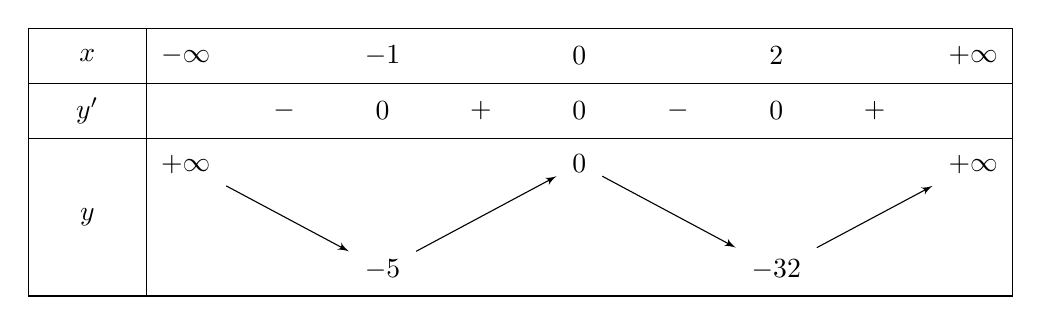
\begin{tikzpicture}
			\tkzTabInit[lgt=1.5,espcl=2.5,deltacl=.5]
			{$x$ /.7, $y’$ /.7,$y$ /2}
			{$-\infty$ , $-1$ , $0$ , $2$ , $+\infty$}
			\tkzTabLine{ ,-,$0$,+,$ 0 $,-,$ 0 $,+, }
			\tkzTabVar{+/$+\infty$ ,-/ $-5$ ,+/$0$, -/$-32$,+/$+\infty$}
			\end{tikzpicture}
		\end{center}
		Hàm số $y= \left|f(x) + m \right|  $ có 7 cực trị khi và chỉ khi $y=f(x)+m$ cắt trục hoành tại $4$ điểm phân biệt. Hay, đồ thị hàm số $y=f(x)$ cắt $y=-m$ tại $4$ điểm phân biệt.\\
		Điều này tương đương với $-5<-m<0$  hay $0<m<5$.\\
		Vậy có 4 giá trị nguyên của $ m  $ để hàm số đã cho có 7 cực trị.
	}
\end{ex}	
\subsection{Hiện (mặc định luôn hiện)}
\showtextchoice
\begin{ex}
	Có bao nhiêu giá trị nguyên của tham số $ m $ để hàm số $ y = \left|3x^4 - 4x^3 - 12x^2 + m \right| $ có 7 điểm cực trị?
	\choice
	{$ 3 $}	
	{$ 5 $}
	{\True $ 4 $}
	{$ 6 $}
	\loigiai{
		Xét $ f(x) = 3x^4 - 4x^3 - 12x^2  $.\\
		Ta có $ f'(x) =0 \Leftrightarrow  12x^3 - 12x^2 - 24x = 0 \Leftrightarrow \hoac{&x = 0  \\ &x = 2 \\&x = -1.}$
		\begin{center}
			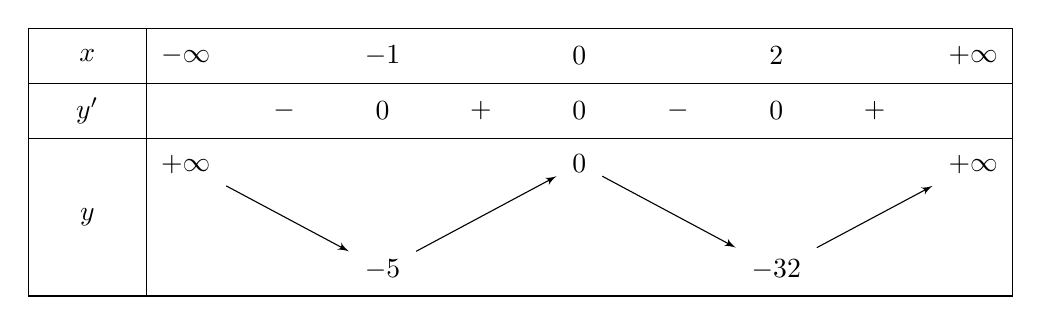
\begin{tikzpicture}
			\tkzTabInit[lgt=1.5,espcl=2.5,deltacl=.5]
			{$x$ /.7, $y’$ /.7,$y$ /2}
			{$-\infty$ , $-1$ , $0$ , $2$ , $+\infty$}
			\tkzTabLine{ ,-,$0$,+,$ 0 $,-,$ 0 $,+, }
			\tkzTabVar{+/$+\infty$ ,-/ $-5$ ,+/$0$, -/$-32$,+/$+\infty$}
			\end{tikzpicture}
		\end{center}
		Hàm số $y= \left|f(x) + m \right|  $ có 7 cực trị khi và chỉ khi $y=f(x)+m$ cắt trục hoành tại $4$ điểm phân biệt. Hay, đồ thị hàm số $y=f(x)$ cắt $y=-m$ tại $4$ điểm phân biệt.\\
		Điều này tương đương với $-5<-m<0$  hay $0<m<5$.\\
		Vậy có 4 giá trị nguyên của $ m  $ để hàm số đã cho có 7 cực trị.
	}
\end{ex}	
\section{Lệnh immini}
\subsection{Mặc định}
\begin{verbatim}
\immini{text}{images}
\end{verbatim}
\begin{dn}
	\immini{
		Điểm $ M(a;b) $ trong một hệ trục tọa độ vuông góc của mặt phẳng được gọi là \textbf{điểm biểu diễn số phức} $ z=a+bi $.
		Giả sử số phức $ z=a+bi $ được biểu diễn bởi điểm $ M(a;b) $ trên mặt phẳng tọa độ.
	}
	{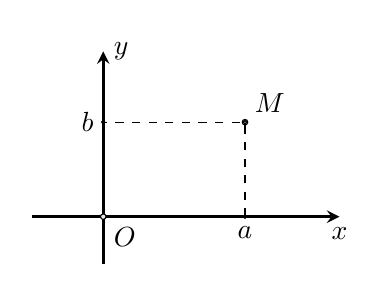
\begin{tikzpicture}[>=stealth,scale=0.6]
		\tkzInit[xmin=-1.6,xmax=5.5, ymin=-1.2, ymax=4]
		\tkzClip
		\draw[->,line width = 1pt] (-1.5,0)--(0,0) node[below right]{$O$}--(5,0) node[below]{$x$};
		\draw[->,line width = 1pt] (0,-1) --(0,3.5) node[right]{$y$};
		\foreach \x in {}{
			\draw (\x,0) node[below]{$\x$} circle (1pt);
			\draw (0,\x) node[left]{$\x$} circle (1pt);
		}
		\tkzDefPoints{0/0/O,3/2/M}
		\tkzDrawPoints(O,M)
		\tkzDefPoints{0/0/A,3/2/B}
		\tkzDrawVectors(A,B)
		\draw (0,2) node[left]{$b$} circle (1pt);
		\draw (3,0) node[below]{$a$} circle (1pt);
		\draw (3,2) node[above right]{$M$} circle (1pt);
		\draw [dashed] (3,0)--(3,2)--(0,2);
		\end{tikzpicture}}
\end{dn}
\subsection{Thêm tham số khoảng cách giữa hình và text}
\begin{verbatim}
\immini[0.4]{text}{images}%0.4 là khoảng cách giữa text và hình chiếm 40% độ rộng khổ giấy
\end{verbatim}
\begin{dn}
	\immini[0.4]{
		Điểm $ M(a;b) $ trong một hệ trục tọa độ vuông góc của mặt phẳng được gọi là \textbf{điểm biểu diễn số phức} $ z=a+bi $.
		Giả sử số phức $ z=a+bi $ được biểu diễn bởi điểm $ M(a;b) $ trên mặt phẳng tọa độ.
	}
	{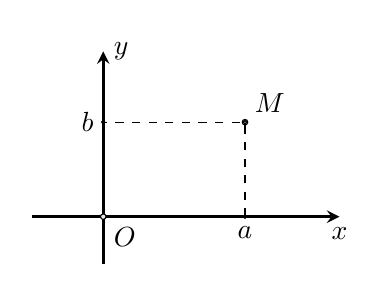
\begin{tikzpicture}[>=stealth,scale=0.6]
		\tkzInit[xmin=-1.6,xmax=5.5, ymin=-1.2, ymax=4]
		\tkzClip
		\draw[->,line width = 1pt] (-1.5,0)--(0,0) node[below right]{$O$}--(5,0) node[below]{$x$};
		\draw[->,line width = 1pt] (0,-1) --(0,3.5) node[right]{$y$};
		\foreach \x in {}{
			\draw (\x,0) node[below]{$\x$} circle (1pt);
			\draw (0,\x) node[left]{$\x$} circle (1pt);
		}
		\tkzDefPoints{0/0/O,3/2/M}
		\tkzDrawPoints(O,M)
		\tkzDefPoints{0/0/A,3/2/B}
		\tkzDrawVectors(A,B)
		\draw (0,2) node[left]{$b$} circle (1pt);
		\draw (3,0) node[below]{$a$} circle (1pt);
		\draw (3,2) node[above right]{$M$} circle (1pt);
		\draw [dashed] (3,0)--(3,2)--(0,2);
		\end{tikzpicture}}
\end{dn}
\subsection{Tương thích giữa lệnh immini với môi trường liệt kê}
\subsubsection{Cách 1: ý đầu và hình đặt ngang hàng với nhau}
\begin{ex}[Đề thi vào 10, Sở giáo dục Bà Rịa - Vũng Tàu, 2016]%[9D4B2]%[9D2B3]
	\begin{enumerate}    
		\item Vẽ parabol $(P):y=\dfrac{1}{2}x^2 $.
		\item Tìm giá trị của $m$ để đường thẳng $(d):y = 2x + m$  đi qua điểm  $M(2;3)$.
	\end{enumerate}
	\loigiai
	{
		\begin{enumerate}
			\item 	
			\immini{	
				Bảng giá trị của hàm số $y=\dfrac{1}{2}x^2$ là:
				\begin{center}
					\begin{tabular}{|c|c|c|c|c|c|}
						\hline 
						$x$ & $-4$ & $-2$	& $0$ & $2$ & $4$ \\ 
						\hline 
						$y=\dfrac{1}{2}x^2$ & $8$ & $2$ & $0$ & $2$ & $8$\\ 
						\hline
					\end{tabular}
				\end{center}
				Đồ thị như hình bên
			}
			{	
				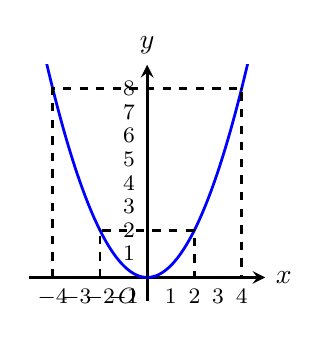
\begin{tikzpicture}[line width=1pt,>=stealth,x=1cm,y=1cm,scale=0.3]
				%\draw[thin,color=gray!50] (-4,-1) grid (4,5);        				
				\draw[->] (-5,0) -- (5,0) node[right] {$x$};
				\foreach \x in {-4,-3,-2,-1,1,2,3,4} 
				\draw[shift={(\x,0)},color=black] (0pt,2pt) -- (0pt,-2pt) node[below] {\footnotesize $\x$};       	
				\draw[->] (0,-1) -- (0,9) node[above] {$y$};
				\foreach \y in {1,2,3,4,5,6,7,8}
				\draw[shift={(0,\y)},color=black] (2pt,0pt) -- (-2pt,0pt) node[left] {\footnotesize $\y$};
				\draw (0,0) node[below left]{\footnotesize $O$};
				\clip (-5,-1) rectangle (5,9);        				
				\draw[samples=200,color=blue]   plot (\x,{1/2*(\x)^2});
				\draw[dashed] (-4,0) -- (-4,8) -- (4,8) -- (4,0);
				\draw[dashed] (-2,0) -- (-2,2) -- (2,2) -- (2,0);
				\fill (0,0) circle (1.5pt);        				
				\fill (-4,8) circle (1.5pt);
				\fill (-2,2) circle (1.5pt);
				\fill (2,2) circle (1.5pt);
				\fill (4,8) circle (1.5pt);   				
				\end{tikzpicture}
			}      
			\item Vì đường thẳng $(d):y = 2x + m$  đi qua điểm  $M(2;3)$ nên ta có: $3=2.2+m \Leftrightarrow m=-1$.\\
			Vậy $m=-1$.
		\end{enumerate} 		
	}
\end{ex}
\subsubsection{Cách 2: mọi ý đều đặt ngang hàng với hình}
\begin{ex}[Đề thi vào 10, Sở giáo dục Bà Rịa - Vũng Tàu, 2016]%[9D4B2]%[9D2B3]
	\begin{enumerate}    
		\item Vẽ parabol $(P):y=\dfrac{1}{2}x^2 $.
		\item Tìm giá trị của $m$ để đường thẳng $(d):y = 2x + m$  đi qua điểm  $M(2;3)$.
	\end{enumerate}
	\loigiai
	{
		\vspace*{-1cm}
		\immini{	
			\begin{enumerate}
				\item 	
				Bảng giá trị của hàm số $y=\dfrac{1}{2}x^2$ là:
				\begin{center}
					\begin{tabular}{|c|c|c|c|c|c|}
						\hline 
						$x$ & $-4$ & $-2$	& $0$ & $2$ & $4$ \\ 
						\hline 
						$y=\dfrac{1}{2}x^2$ & $8$ & $2$ & $0$ & $2$ & $8$\\ 
						\hline
					\end{tabular}
				\end{center}
				Đồ thị như hình bên
				\item Vì đường thẳng $(d):y = 2x + m$  đi qua điểm  $M(2;3)$ nên ta có: $3=2.2+m \Leftrightarrow m=-1$.\\
				Vậy $m=-1$.
			\end{enumerate}
		}
		{	
			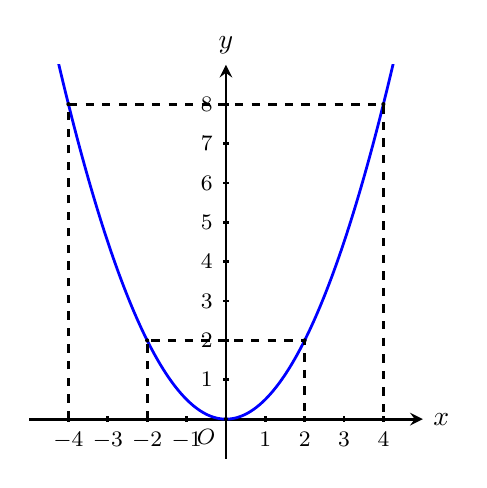
\begin{tikzpicture}[line width=1pt,>=stealth,x=1cm,y=1cm,scale=0.5]
			%\draw[thin,color=gray!50] (-4,-1) grid (4,5);        				
			\draw[->] (-5,0) -- (5,0) node[right] {$x$};
			\foreach \x in {-4,-3,-2,-1,1,2,3,4} 
			\draw[shift={(\x,0)},color=black] (0pt,2pt) -- (0pt,-2pt) node[below] {\footnotesize $\x$};       	
			\draw[->] (0,-1) -- (0,9) node[above] {$y$};
			\foreach \y in {1,2,3,4,5,6,7,8}
			\draw[shift={(0,\y)},color=black] (2pt,0pt) -- (-2pt,0pt) node[left] {\footnotesize $\y$};
			\draw (0,0) node[below left]{\footnotesize $O$};
			\clip (-5,-1) rectangle (5,9);        				
			\draw[samples=200,color=blue]   plot (\x,{1/2*(\x)^2});
			\draw[dashed] (-4,0) -- (-4,8) -- (4,8) -- (4,0);
			\draw[dashed] (-2,0) -- (-2,2) -- (2,2) -- (2,0);
			\fill (0,0) circle (1.5pt);        				
			\fill (-4,8) circle (1.5pt);
			\fill (-2,2) circle (1.5pt);
			\fill (2,2) circle (1.5pt);
			\fill (4,8) circle (1.5pt);   				
			\end{tikzpicture}
		}       		
	}
\end{ex}
\subsubsection{Cách 3: 2 ý đầu đặt ngang hàng với hình, ý 3 đặt độc lập}
\begin{ex}[Đề thi vào 10, Sở giáo dục Bà Rịa - Vũng Tàu, 2016]%[9D4B2]%[9D2B3]
	\begin{enumerate}    
		\item Vẽ parabol $(P):y=\dfrac{1}{2}x^2 $.
		\item Tìm giá trị của $m$ để đường thẳng $(d):y = 2x + m$  đi qua điểm  $M(2;3)$.
		\item Câu hỏi ý 3
	\end{enumerate}
	\loigiai
	{
		\vspace*{-1cm}
		\immini{	
			\begin{enumerate}
				\item 	
				Bảng giá trị của hàm số $y=\dfrac{1}{2}x^2$ là:
				\begin{center}
					\begin{tabular}{|c|c|c|c|c|c|}
						\hline 
						$x$ & $-4$ & $-2$	& $0$ & $2$ & $4$ \\ 
						\hline 
						$y=\dfrac{1}{2}x^2$ & $8$ & $2$ & $0$ & $2$ & $8$\\ 
						\hline
					\end{tabular}
				\end{center}
				Đồ thị như hình bên
				\item Vì đường thẳng $(d):y = 2x + m$  đi qua điểm  $M(2;3)$ nên ta có: $3=2.2+m \Leftrightarrow m=-1$.\\
				Vậy $m=-1$.
			\end{enumerate}
		}
		{	
			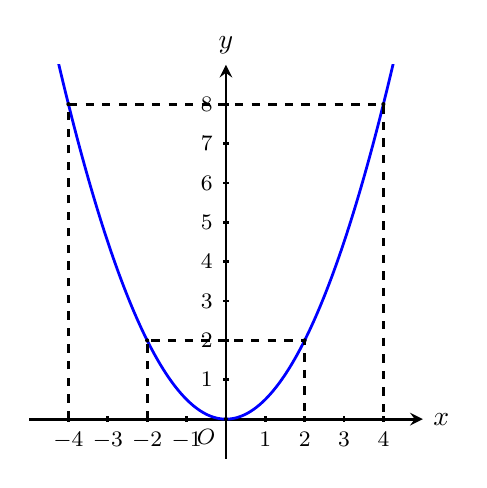
\begin{tikzpicture}[line width=1pt,>=stealth,x=1cm,y=1cm,scale=0.5]
			%\draw[thin,color=gray!50] (-4,-1) grid (4,5);        				
			\draw[->] (-5,0) -- (5,0) node[right] {$x$};
			\foreach \x in {-4,-3,-2,-1,1,2,3,4} 
			\draw[shift={(\x,0)},color=black] (0pt,2pt) -- (0pt,-2pt) node[below] {\footnotesize $\x$};       	
			\draw[->] (0,-1) -- (0,9) node[above] {$y$};
			\foreach \y in {1,2,3,4,5,6,7,8}
			\draw[shift={(0,\y)},color=black] (2pt,0pt) -- (-2pt,0pt) node[left] {\footnotesize $\y$};
			\draw (0,0) node[below left]{\footnotesize $O$};
			\clip (-5,-1) rectangle (5,9);        				
			\draw[samples=200,color=blue]   plot (\x,{1/2*(\x)^2});
			\draw[dashed] (-4,0) -- (-4,8) -- (4,8) -- (4,0);
			\draw[dashed] (-2,0) -- (-2,2) -- (2,2) -- (2,0);
			\fill (0,0) circle (1.5pt);        				
			\fill (-4,8) circle (1.5pt);
			\fill (-2,2) circle (1.5pt);
			\fill (2,2) circle (1.5pt);
			\fill (4,8) circle (1.5pt);   				
			\end{tikzpicture}
		}       		
		\begin{enumerate}
			\item[3.] Lời giải ý 3 đặt riêng,... Lời giải ý 3 đặt riêng,... Lời giải ý 3 đặt riêng,... Lời giải ý 3 đặt riêng,... Lời giải ý 3 đặt riêng,... Lời giải ý 3 đặt riêng,... Lời giải ý 3 đặt riêng,... 
		\end{enumerate}
	}
\end{ex}
\section{Tự động break xuống dòng mới khi bắt đầu môi trường bài tập, ví dụ là các môi trường liệt kê}
Mặc định chỉ áp dụng với môi trường \{ex\}, với các môi trường ví dụ (vd), bài tập (bt),... cần có khai báo
\begin{center}
\begin{verbatim}
\listenumerate{vd,bt}
\end{verbatim}
\end{center}
\begin{ex}[Đề thi vào 10, Sở giáo dục Bà Rịa - Vũng Tàu, 2016]%[9D4B2]%[9D2B3]
    \begin{enumerate}    
        \item Vẽ parabol $(P):y=\dfrac{1}{2}x^2 $.
        \item Tìm giá trị của $m$ để đường thẳng $(d):y = 2x + m$  đi qua điểm  $M(2;3)$.
    \end{enumerate}
\loigiai
    {
    \begin{enumerate}
        \item Bảng giá trị của hàm số $y=\dfrac{1}{2}x^2$ là:
        		\begin{center}
        			\begin{tabular}{|c|c|c|c|c|c|}
        			\hline 
        			$x$ & $-4$ & $-2$	& $0$ & $2$ & $4$ \\ 
        			\hline 
        			$y=\dfrac{1}{2}x^2$ & $8$ & $2$ & $0$ & $2$ & $8$\\ 
        			\hline
        			\end{tabular}
        		\end{center}
        		Đồ thị:
        		\begin{center}
        			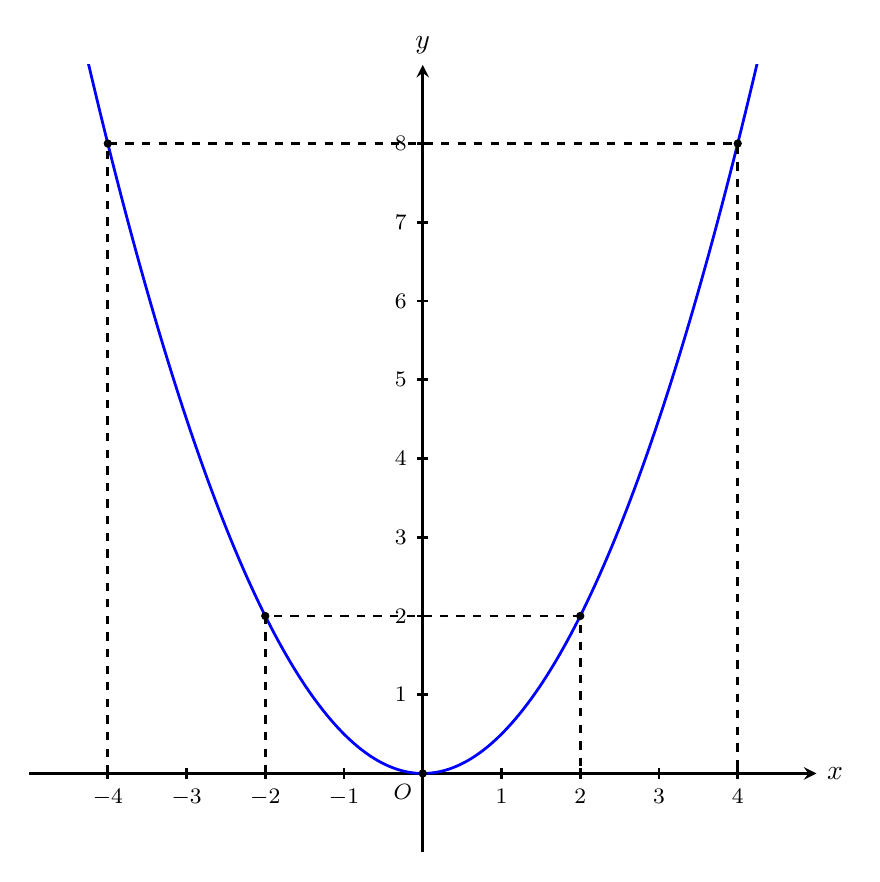
\begin{tikzpicture}[line width=1pt,>=stealth,x=1cm,y=1cm,scale=1]
        				%\draw[thin,color=gray!50] (-4,-1) grid (4,5);        				
        				\draw[->] (-5,0) -- (5,0) node[right] {$x$};
        				\foreach \x in {-4,-3,-2,-1,1,2,3,4} 
        				\draw[shift={(\x,0)},color=black] (0pt,2pt) -- (0pt,-2pt) node[below] {\footnotesize $\x$};       	
        				\draw[->] (0,-1) -- (0,9) node[above] {$y$};
        				\foreach \y in {1,2,3,4,5,6,7,8}
        				\draw[shift={(0,\y)},color=black] (2pt,0pt) -- (-2pt,0pt) node[left] {\footnotesize $\y$};
        				\draw (0,0) node[below left]{\footnotesize $O$};
        				\clip (-5,-1) rectangle (5,9);        				
        				\draw[samples=200,color=blue]   plot (\x,{1/2*(\x)^2});
        				\draw[dashed] (-4,0) -- (-4,8) -- (4,8) -- (4,0);
        				\draw[dashed] (-2,0) -- (-2,2) -- (2,2) -- (2,0);
        				\fill (0,0) circle (1.5pt);        				
        				\fill (-4,8) circle (1.5pt);
        				\fill (-2,2) circle (1.5pt);
        				\fill (2,2) circle (1.5pt);
        				\fill (4,8) circle (1.5pt);   				
        			\end{tikzpicture}
        		\end{center}        		
        \item Vì đường thẳng $(d):y = 2x + m$  đi qua điểm  $M(2;3)$ nên ta có: $3=2.2+m \Leftrightarrow m=-1$.\\
        		Vậy $m=-1$.
    \end{enumerate}
    }
\end{ex}
\section{Thêm tùy chọn solcolor}
Tùy chọn \textbf{loigiai} chỉ in lời giải, không in đáp án chi tiết.\\
Tùy chọn \textbf{solcolor} vừa in lời giải vừa in đáp án chi tiết.
\section{Định nghĩa lại dấu kết thúc lời giải}
\begin{verbatim}
\def\qedEX{Kí hiệu muốn đặt là dấu kết thúc môi trường loigiai}
\end{verbatim}
\def\qedEX{\color{blue}\ensuremath{\square}}
\section{Hiện đáp số vắn tắt bài tập tự luận}
\begin{verbatim}
\Opensolutionfile{ansshort}[ans/ansshort1]
\begin{ex}
NỘI DUNG CÂU HỎI
\loigiai
{
NỘI DUNG LỜI GIẢI CHI TIẾT
}
\shortsol
{
NỘI DUNG ĐÁP SỐ VẮN TẮT
}
\end{ex}
.
.
.
\Closesolutionfile{ansshort}
\end{verbatim}
\begin{ex}
	Một xưởng sản xuất gỗ cưa các khúc gỗ thành
	các tấm ván. Có hai loại ván: ván thành phẩm và ván sử dụng trong xây
	dựng. Giả sử, đối với:
	
	Ván thành phẩm cần $1$ giờ để cưa và $3$ giờ để bào $10$m ván.
	
	Ván xây dựng cần $2$ giờ để cưa và $2$ giờ để bào $10$m ván.
	
	Máy cưa làm việc tối đa $3$ giờ trong ngày, và máy bào làm việc tối đa $5$ giờ
	trong ngày. Nếu lợi nhuận của $10$m ván thành phẩm là $100$ (ngàn đồng) và
	lợi nhuận của $10$m ván xây dựng là $80$ (ngàn đồng). Trong ngày, xưởng sản xuất 
	phải cưa bao nhiêu ván mỗi loại để lợi nhuận lớn nhất?
\loigiai{
		\immini{Gọi $x,y$ lần lượt là chiều dài ván thành phẩm và ván xây dựng hoàn thành trong một ngày. Đơn vị $10$m. Do đó bài toán trở thành tìm giá trị lớn nhất của $T=10x+8y$ (ngàn đồng), biết $x,y$ thỏa mãn hệ bất phương trình sau
			\begin{center}
				$\left\{ \begin{aligned}
				x+2y &\le 3 \\ 
				3x+2y & \le 5 \\
				x& \ge 0\\ 
				y &\ge 0.
				\end{aligned} \right.$
			\end{center}
		}{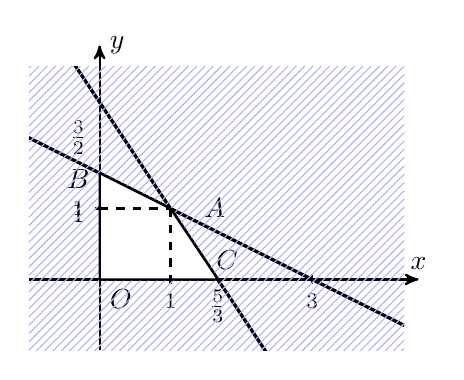
\begin{tikzpicture}[scale=0.9,thick,>=stealth']
			\draw[->] (-1,0) -- (4.5,0) node[above]{$x$};
			\foreach \x in {1,3}
			\draw[shift={(\x,0)},color=black] (0pt,2pt) -- (0pt,-2pt) node[below] {\footnotesize $\x$};
			\draw[->,color=black] (0,-1) -- (0,3.3)node[right]{$y$};
			\foreach \y in {1}
			\draw[shift={(0,\y)},color=black] (2pt,0pt) -- (-2pt,0pt) node[left] {\footnotesize $\y$};
			\node[below right] at (0,0) {$O$};
			\node[below ] at (1.667,0) {$\frac{5}{3}$};	
			\node[right=0.3] at (1,1) {$A$};	
			\node at (-0.3,2.) {$\frac{3}{2}$};
			\node[below ] at (-0.3,1.7) {$B$};	
			\node[below ] at (-0.3,1.2) {$1$};	
			\node[above ] at (1.8,0) {$C$};			
			%\draw[fill]  (4,0) circle (1.5pt) (0,0) circle (1.5pt) (2,2) circle (1.5pt);
			\clip(-1.0,-1) rectangle (4.3,3.0);		
			\draw[line width=1.2pt,smooth,samples=100,domain=-1.0:4.3] plot(\x,{1.5-
				0.5*(\x)});
			\draw[line width=1.2pt,smooth,samples=100,domain=-1.0:4.3] plot(\x,{2.5-1.5*(\x)});
			\fill[pattern=north east lines,pattern color=blue!30] (-1,-1) -- (-1,3) -- (5,3) -- (5,-1) -- cycle;
			\fill[white] (0,0) -- (0,1.5) -- (1,1)--(1.667,0) -- cycle;   
			\draw[dashed] (0,1)--(1,1) (1,1)--(1,0);
			\draw (0,1.5)--(0,0) -- (1.667,0) -- (1,1)--(0,1.5); 
			\end{tikzpicture}}
			Miền nghiệm của hệ là tứ giác $OBAC$, trong đó
			$A(1;1),B\left(0;\dfrac{3}{2}\right), C\left(\dfrac{5}{3};0\right).$
			Do đó, giá trị lớn nhất của $T$ là $18$ khi $x=y=1.$
	}
\shortsol{
 $\max T= 18$.
}
\end{ex}

\begin{ex}
Tứ diện đều có bao nhiêu mặt phẳng đối xứng?
\loigiai
{
NỘI DUNG LỜI GIẢI CHI TIẾT 
}
\shortsol{6}
\end{ex}
\begin{ex}
Cho hình chóp $S.ABC$ có đáy $ABC$ là tam giác vuông cân tại $B$, cạnh $AB=3$. Cạnh bên $SA=4$ và vuông góc với mặt phẳng đáy. Tính bán kính mặt cầu ngoại tiếp hình chóp $S.ABC$ là
\loigiai
{
NỘI DUNG LỜI GIẢI CHI TIẾT 
}
\shortsol{$\dfrac{\sqrt{34}}2$}
\end{ex}
\begin{ex}
Biết tập nghiệm của phương trình $\log_3\left( \sqrt{x^2+x+2}+1 \right)+3\log_3\left( x^2+x+3 \right)<4$ là $\left( a;b \right).$ Tính tổng $2a+b$? \loigiai
{
NỘI DUNG LỜI GIẢI CHI TIẾT 
}
\shortsol{$-3$}
\end{ex}
\begin{ex}
Cho $A$,$B$,$C$ tương ứng là các điểm trong mặt phẳng phức biểu diễn các số phức $z_1=-1-2i$, $z_2=2-5i$, $z_3=-2-4i$. Số phức $z$ biểu diễn bởi điểm $D$ sao cho $ABCD$ là hình bình hành. Tìm $z$.
\loigiai
{
NỘI DUNG LỜI GIẢI CHI TIẾT 
}
\shortsol{$-5-i$}
\end{ex}
\begin{ex}
Viết phương trình tiếp tuyến của đồ thị hàm số $y=-2x^3+8x+2$ tại điểm có hoành độ bằng $0$.
\loigiai
{
NỘI DUNG LỜI GIẢI CHI TIẾT 
}
\shortsol{$y=8x+2$}
\end{ex}
\Closesolutionfile{ansshort}
\begin{center}
\textbf{ĐÁP SỐ CÂU HỎI TỰ LUẬN MẶC ĐỊNH}
\end{center}
\begin{flushleft}
\input{ans/ansshort1} 
\end{flushleft}
%%%
\begin{center}
\textbf{ĐÁP SỐ CÂU HỎI TỰ LUẬN HAI CỘT}
\end{center} 
\shortsolnum{2}
\begin{flushleft}
\input{ans/ansshort1} 
\end{flushleft}
\section{Các ví dụ luôn ẩn lời giải}
Cấu trúc lệnh
\begin{verbatim}
\hideansEX{vd}%luôn ẩn lời giải
Có thể thay môi trường vd bởi môi trường ex hoặc môi trưởng bt hoặc môi trường 
bất kì đã được định nghĩa sẵn
\end{verbatim}
\hideansEX{vd}%luôn ẩn lời giải
\begin{vd}%[Đề tham khảo BGD 2017-2018]%[2H3G2]
	Trong không gian $ Oxyz, $ cho điểm $ M(1;1;2) $. Hỏi có bao nhiêu mặt phẳng $ (P) $ đi qua $ M $ và cắt các trục $ x'Ox, y'Oy, z'Oz $ lần lượt tại các điểm $ A, B, C $ sao cho $ OA = OB = OC \ne 0? $
	\choice
	{\True $ 3 $}
	{$ 1 $}
	{$ 4 $}
	{$ 8 $}
	\loigiai
	{
		Giả sử $ A(a,0,0), B(0,b,0), C(0,0,c) $\, (với $ a,b,c \ne 0 $).\\
		Mặt phẳng $ (P): \dfrac{x}{a} + \dfrac{y}{b} + \dfrac{z}{c} = 1 $.\\
		Do điểm $ M $ thuộc $ (P) $ nên ta có $ \dfrac{1}{a} + \dfrac{1}{b} + \dfrac{2}{c} = 1$ $(*)$.\\
		Mặt khác $ OA = OB = OC  $ nên $ |a| =|b|=|c|  $.
		\begin{itemize}
			\item Trường hợp $ b=a$ và $c=a$.\\
			Kết hợp với $(*)$ ta được: $\dfrac{1}{a} + \dfrac{1}{a} + \dfrac{2}{a} = 1\Leftrightarrow a = 4$. Suy ra $ b = c=a=4. $\\
			Mặt phẳng lúc đó là: $ (P): \dfrac{x}{4} + \dfrac{y}{4} + \dfrac{z}{4} = 1 $.
			\item Trường hợp $ b=a$ và $c=-a$. \\
			Khi đó: $\dfrac{1}{a} +\dfrac{1}{a} - \dfrac{2}{a} = 1$, vô lý.
			\item Trường hợp $ b=-a$ và $c=a$.\\
			Trường hợp này ta tìm được $ a = 2 = c, b = -2 $. \\
			Và $ (P): \dfrac{x}{2} + \dfrac{y}{-2} + \dfrac{z}{2} = 1 $.
			\item Trường hợp $b=-a$ và $c=-a$.\\
			Trường hợp này ta tìm được $ a = -2, b = c = 2 $.\\
			Và $ (P): \dfrac{x}{-2} + \dfrac{y}{2} + \dfrac{z}{2} = 1 $.
		\end{itemize}
		Vậy có tất cả ba mặt phẳng thỏa mãn đề bài.
	}
\end{vd}		

\section{Các bài tập tự luyện luôn ẩn lời giải và hiện dòng kẻ}
Cấu trúc lệnh
\begin{verbatim}
\dotlineans{5}{bt}%luôn ẩn lời giải và hiện 5 dòng kẻ
\end{verbatim}
\dotlineans{5}{bt}%luôn ẩn lời giải và hiện 5 dòng kẻ
\begin{bt}
	Có bao nhiêu giá trị nguyên của tham số $ m $ để hàm số $ y = \left|3x^4 - 4x^3 - 12x^2 + m \right| $ có 7 điểm cực trị?
	\choice
	{$ 3 $}	
	{$ 5 $}
	{\True $ 4 $}
	{$ 6 $}
	\loigiai{
		Xét $ f(x) = 3x^4 - 4x^3 - 12x^2  $.\\
		Ta có $ f'(x) =0 \Leftrightarrow  12x^3 - 12x^2 - 24x = 0 \Leftrightarrow \hoac{&x = 0  \\ &x = 2 \\&x = -1.}$
		\begin{center}
			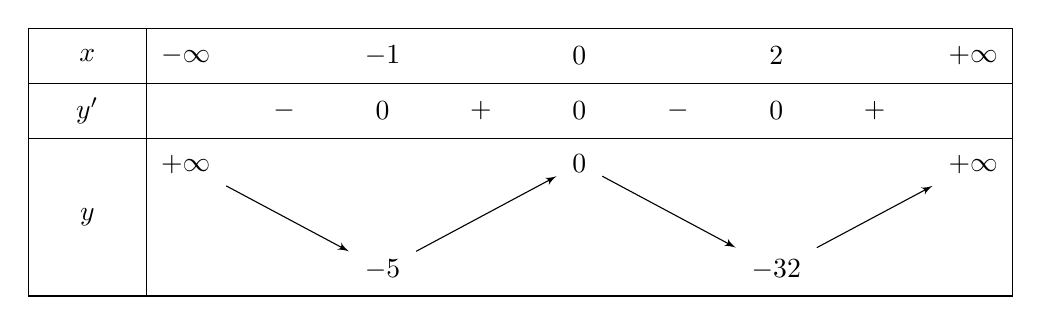
\begin{tikzpicture}
			\tkzTabInit[lgt=1.5,espcl=2.5,deltacl=.5]
			{$x$ /.7, $y’$ /.7,$y$ /2}
			{$-\infty$ , $-1$ , $0$ , $2$ , $+\infty$}
			\tkzTabLine{ ,-,$0$,+,$ 0 $,-,$ 0 $,+, }
			\tkzTabVar{+/$+\infty$ ,-/ $-5$ ,+/$0$, -/$-32$,+/$+\infty$}
			\end{tikzpicture}
		\end{center}
		Hàm số $y= \left|f(x) + m \right|  $ có 7 cực trị khi và chỉ khi $y=f(x)+m$ cắt trục hoành tại $4$ điểm phân biệt. Hay, đồ thị hàm số $y=f(x)$ cắt $y=-m$ tại $4$ điểm phân biệt.\\
		Điều này tương đương với $-5<-m<0$  hay $0<m<5$.\\
		Vậy có 4 giá trị nguyên của $ m  $ để hàm số đã cho có 7 cực trị.
	}
\end{bt}		

\begin{bt}
	Trong không gian $ Oxyz,  $	cho điểm $ A(2;2;1) $, $ B\left(-\dfrac{8}{3}; \dfrac{4}{3};\dfrac{8}{3}\right). $ Đường thẳng đi qua tâm đường tròn nội tiếp của tam giác $ OAB $ và vuông góc với mặt phẳng $ (OAB) $ có phương trình là
	\choice
	{\True $ \dfrac{x+1}{1} = \dfrac{y-3}{-2} = \dfrac{z+1}{2} $}	
	{$ \dfrac{x+1}{1} = \dfrac{y-3}{-2} = \dfrac{z-4}{2} $}
	{ $ \dfrac{x+\tfrac{1}{3}}{1} = \dfrac{y-\tfrac{5}{3}}{-2} = \dfrac{z-\tfrac{11}{6}}{2} $}
	{$ \dfrac{x+\tfrac{2}{9}}{1} = \dfrac{y-\tfrac{2}{9}}{-2} = \dfrac{z+\tfrac{5}{9}}{2} $}
	\loigiai{
		Mặt phẳng $ (OAB) $	 có véc-tơ pháp tuyến là $ \vec{n} = (1; -2;2) $ nên đường thẳng $ d $ cần tìm có VTCP $ \vec{u} = (1; -2;2)$.
		Gọi $ I $ là tâm đường tròn nội tiếp tam giác $ OAB $. \\
	Khi đó ta có $ BO \cdot \vec{IA} + OA \cdot \vec{IB} + AB \cdot \vec{IO} = \vec{0} \Rightarrow \heva{x_I = \dfrac{BO \cdot x_A + OA \cdot x_B + AB \cdot x_O}{BO + OA + AB} \\y_I = \dfrac{BO \cdot y_A + OA \cdot y_B + AB \cdot y_O}{BO + OA + AB} \\ z_I = \dfrac{BO \cdot z_A + OA \cdot z_B + AB \cdot z_O}{BO + OA + AB}}  \Rightarrow I(0;1;1).$\\
	Vậy phương trình đường thẳng cần tìm $ \dfrac{x+1}{1} = \dfrac{y-3}{-2} = \dfrac{z+1}{2} $.
}
\end{bt}		
\begin{bt}
	Cho hai hình vuông $ ABCD $	và $ ABEF $ có cạnh bằng $ 1 $, lần lượt nằm trên hai mặt phẳng vuông góc với nhau. Gọi $ S $ là điểm đối xứng với $ B $ qua đường thẳng $ DE $. Tính thể tích của khối da diện $ ABCDSEF $.
	\choice
	{$ \dfrac{7}{6} $}	
	{$ \dfrac{11}{12} $}
	{$ \dfrac{2}{3} $}
	{\True $ \dfrac{5}{6} $}
	\loigiai
	{Chọn hệ trục tọa độ sao cho hình vuông $ ABCD $ trên mp$ (Oxy)$, hình vuông $ ABEF $ nằm trên mặt phẳng $ (Oxz) $ và $ A $ trùng gốc tọa độ. Khi đó $ A(0;0;0), B(1;0;0), D(0;1;0), F(0;0;1) $	suy ra $ E(1;0;1). $
		\begin{center}
		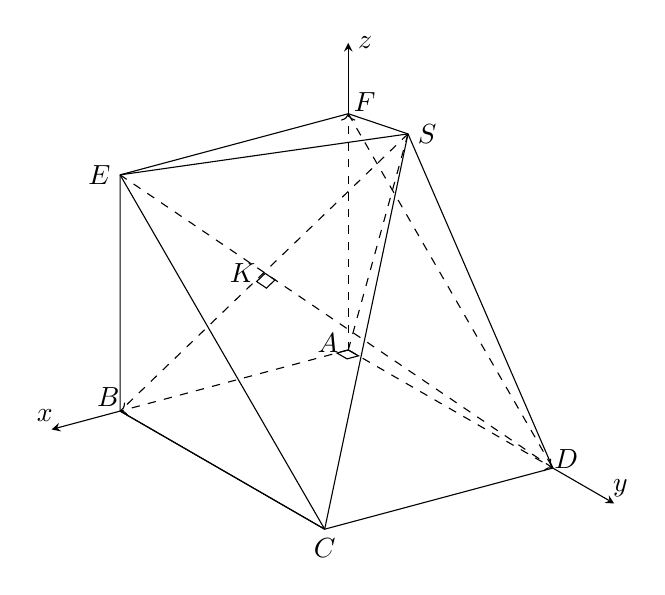
\begin{tikzpicture}
		[x={({sin(-75)*1cm},{-cos(75)*1cm})},y={(0.866cm,-0.5cm)},z={(0cm,1cm)},scale = 3]
		\coordinate (a) at (0,0,0);
		\coordinate (d) at (0,1,0);
		\coordinate (b) at (1,0,0);
		\coordinate (k) at (0.66,0.33,0.66);
		\draw [->,dashed] (0,0,0)--(1,0,0) ;
		\draw [->,dashed] (0,0,0)--(0,1,0) ;
		\draw [->,dashed] (0,0,0)--(0,0,1) ;
				\draw [>=stealth] (1,0,0)--(1,1,0);
				\draw [>=stealth] (1,0,0)--(1,1,0)--(0,1,0)--(0.33,0.66,1.33)--(1,0,1)--(1,0,0);
				\draw [>=stealth] (0.33,0.66,1.33)--(0,0,1)--(1,0,1);
				\draw [>=stealth] (0.33,0.66,1.33)--(1,1,0);
		\draw [dashed] (0.33,0.66,1.33)--(1,0,0);
		\draw [dashed] (0.33,0.66,1.33)--(0,0,0);
		\draw [dashed] (0,1,0)--(1,0,1);
		\draw (1,0,1)--(1,1,0);
		\node at (0,0,0.03) [left] {$ A $};
		\node at (0.96,0,0.05) [left] {$ B $};
		\node at (0,0.96,0.02) [right] {$ D $};
		\node at (0,-0.02,1.04) [right] {$ F $};
		\node at (1,0,1) [left] {$ E $};
		\node at (1,1,0) [right, below] {$ C $};
		\draw[>=stealth,->] (1,0,0)--(1.3,0,0) node [pos = 1.1][above] {$ x $};
		\draw [>=stealth,->] (0,1,0)--(0,1.3,0) node [pos = 1.1] [above]{$ y $};
		\draw[>=stealth,->] (0,0,1)--(0,0,1.3) node [pos = 1] [right]{$ z $};
		\draw [>=stealth,dashed] (0,0,1)--(0,1,0);
		\node at (0.66,0.33,0.66) [left] {$ K $};
		\node at (0.33,0.66,1.33) [right] {$ S $};
		\tkzMarkRightAngle[size=0.05](d,k,b);
		\tkzMarkRightAngle[size=0.05](d,a,b);
			\end{tikzpicture}
		\end{center} 
		Phương trình đường thẳng $ DE: \heva{&x = t \\&y = 1-t\\&z = t. } $\\
		Mặt phẳng $ (P) $ qua $ B $ và vuông góc $ DE $ cắt $ DE $ tại $ K $ có phương trình $ x - y + z - 1 = 0$.\\
		$ \Rightarrow K = DE \cap (P) $  có tọa độ là $ K = \left(\dfrac{2}{3}; \dfrac{1}{3}; \dfrac{2}{3}\right) $.\\
		Do $ S $ là điểm đối xứng của $ B $ qua $ DE $ nên $ S =  \left(\dfrac{1}{3}; \dfrac{2}{3}; \dfrac{4}{3}\right) $.
		\begin{itemize}
			\item 		Cách 1: $ V = V_{SABCD} + V_{SABEF} + V_{SADF}+V_{SBCE}= \dfrac{1}{3} \cdot \dfrac{4}{3} + \dfrac{1}{3} \cdot \dfrac{2}{3} + \dfrac{1}{3} \cdot \dfrac{1}{2} \cdot \dfrac{1}{3} + \dfrac{1}{3} \cdot \dfrac{1}{2} \cdot \dfrac{2}{3} = \dfrac{5}{6} $.
			\item Cách 2: Thể tích khối đa diện $ ABCDSEF  $ là $ V_{ABCDSEF} = V_{SCDFE} + V_{ABCDEF}.$\\
			Trong đó: 
			$V_{SCDFE} = \dfrac{1}{3} d\left(S,(CDFE)\right) \cdot S_{CDFE} = \dfrac{1}{3} \cdot \dfrac{1}{\sqrt{2}} \cdot \sqrt{2} = \dfrac{1}{3} $ và $ V_{ABCDEF} = \dfrac{1}{2} $.
		\end{itemize}
		Vậy thể tích cần tìm là $ V = \dfrac{1}{3} + \dfrac{1}{2} = \dfrac{5}{6}.$ 
	}
\end{bt}		

\section{Các bài tập luôn hiện lời giải}
\begin{ex}	
	Cho dãy số $ (u_n) $	thỏa mãn $ \log u_1 +\sqrt{2 + \log u_1 - 2 \log u_{10} } = 2 \log u_{10}$ và $ u_{n+1} = 2u_n $ với mọi $ n \ge 1. $ Giá trị nhỏ nhất của $ n $ để $ u_n > 5^{100} $ bằng
	\choice
	{$247$}
	{\True $248$}
	{$229$}
	{$290$}
	\loigiai
	{
		Ta có $ u_{n+1} = 2u_n \Rightarrow u_{10} =2^9 u_1.   $ \\ Suy ra $ \log u_1 +\sqrt{2 + \log u_1 -2 \log (2^9 u_1)} = 2 \log (2^9 u_1) $ \\
		hay $ \sqrt{2 - 18 \log 2 - \log u_1} = 18 \log 2 + \log u_1 $ \, (điều kiện $ \log u_1 > -18 \log 2 $) \\
		$ \Rightarrow \left(\log u_1\right)^2 + \left(36 \log 2 + 1\right) \cdot \log u_1 -2 +18 \log 2 = 0 \Rightarrow \hoac{&\log u_1 \simeq -4,4 \, \text{ (nhận)} \\&\log u_1 \simeq -7,5 \, \text{ (loại)}  } $\\
		Mặt khác để $ u_n > 5^{100}  \Leftrightarrow 2^{n-1} u_1 >5^{100} \Leftrightarrow n > 100 \log_2 5 - \log u_1 \cdot \log_2 10 + 1 $.\\
		Do $ n  $  là số nguyên nên giá trị nhỏ nhất của $ n  $ là 248.
	}
\end{ex}

Cấu trúc lệnh
\begin{verbatim}
\showansEX{ex}%luôn hiện lời giải
\end{verbatim}
\showansEX{ex}%luôn hiện lời giải
\begin{ex}	
	Cho dãy số $ (u_n) $	thỏa mãn $ \log u_1 +\sqrt{2 + \log u_1 - 2 \log u_{10} } = 2 \log u_{10}$ và $ u_{n+1} = 2u_n $ với mọi $ n \ge 1. $ Giá trị nhỏ nhất của $ n $ để $ u_n > 5^{100} $ bằng
	\choice
	{$247$}
	{\True $248$}
	{$229$}
	{$290$}
	\loigiai
	{
		Ta có $ u_{n+1} = 2u_n \Rightarrow u_{10} =2^9 u_1.   $ \\ Suy ra $ \log u_1 +\sqrt{2 + \log u_1 -2 \log (2^9 u_1)} = 2 \log (2^9 u_1) $ \\
		hay $ \sqrt{2 - 18 \log 2 - \log u_1} = 18 \log 2 + \log u_1 $ \, (điều kiện $ \log u_1 > -18 \log 2 $) \\
		$ \Rightarrow \left(\log u_1\right)^2 + \left(36 \log 2 + 1\right) \cdot \log u_1 -2 +18 \log 2 = 0 \Rightarrow \hoac{&\log u_1 \simeq -4,4 \, \text{ (nhận)} \\&\log u_1 \simeq -7,5 \, \text{ (loại)}  } $\\
		Mặt khác để $ u_n > 5^{100}  \Leftrightarrow 2^{n-1} u_1 >5^{100} \Leftrightarrow n > 100 \log_2 5 - \log u_1 \cdot \log_2 10 + 1 $.\\
		Do $ n  $  là số nguyên nên giá trị nhỏ nhất của $ n  $ là 248.
	}
\end{ex}

\begin{ex}
	Xét các số phức $z = a+bi \, (a,b \in \mathbb{R})$ thỏa mãn $|z-4-3i| = \sqrt{5}$. Tính $P=a+b$ khi $|z+1-3i|+|z-1+i|$ đạt giá trị lớn nhất.
	\choice
	{\True $P = 10$}
	{$P=4$}
	{$P=6$}
	{$P=8$}
	\loigiai{
		Ta có $|z-4-3i| = \sqrt{5} \Leftrightarrow (a-4)^2+(b-3)^2 = 5 \Leftrightarrow a^2+b^2 = 8a +6b -20.$\\
		Đặt $Q = |z+1-3i|+|z-1+i| = \sqrt{(a+1)^2+(b-3)^2}+\sqrt{(a-1)^2+(b+1)^2}.$\\
		$Q^2 \le (1+1)\left[(a+1)^2+(b-3)^2+(a-1)^2+(b+1)^2\right] = 2\left[2(a^2+b^2)-4b+12\right] = 8(4a+2b-7) \, (1)$.\\
		Mặt khác,
		$4a+2b-7 =  4(a-4)+2(b-3)+15 \le \sqrt{(4^2+2^2)\left[(a-4)^2+(b-3)^2\right]}+15=25 \, (2)$\\
		Từ $(1), \,  (2)$ ta nhận được $Q^2 \le 200.$\\
		Dấu bằng khi và chỉ khi $\heva{& 4a+2a-7=25 \\ & \dfrac{a-4}{4}=\dfrac{b-3}{2}} \Leftrightarrow \heva{& a=6 \\ & b = 4}$. Vậy $P = 10$.
	}
\end{ex}

\begin{ex}
	\immini{Cho hình lăng trụ tam giác đều $ABC.A'B'C'$ có $AB = 2\sqrt{3}$ và $AA' = 2$. Gọi $M,N,P$ lần lượt là trung điểm của các cạnh $A'B',A'C'$ và $BC$ (tham khảo hình vẽ bên). Côsin tạo bởi hai mặt phẳng $(AB'C')$ và mặt phẳng $(MNP)$ bằng
		\motcot
		{$\dfrac{6\sqrt{13}}{65}$}
		{\True $\dfrac{\sqrt{13}}{65}$}
		{$\dfrac{17\sqrt{13}}{65}$}
		{$\dfrac{18\sqrt{13}}{65}$}}{
		\begin{tikzpicture}[line cap=round,line join=round, >=stealth,scale=1]
		\tkzDefPoints{0/0/A, -4/-2/B, 2/-2/C, 0/5/A'}
		\coordinate (B') at ($(A')+(B)-(A)$);
		\coordinate (C') at ($(A')+(C)-(A)$);
		
		\tkzDefMidPoint(A',B') \tkzGetPoint{M}
		\tkzDefMidPoint(A',C') \tkzGetPoint{N}
		\tkzDefMidPoint(B,C) \tkzGetPoint{P}
		
		
		% 
		\tkzDrawSegments[dashed](A,A' A,B A,C P,M P,N)
		\tkzDrawSegments(B,C B,B' C,C' A',B' B',C' A',C' M,N)
		\tkzLabelPoints[below](B,C,P)
		\tkzLabelPoints[above](A',B',C',M,N)
		\tkzLabelPoints[above left](A)
		\end{tikzpicture}
	}
	\loigiai{ 
		
		\immini{
			Gọi $I,Q$ lần lượt là trung điểm của $MN$, $B'C'$. Gọi $O = PI \cap AQ$. Khi đó giao tuyến của $(AB'C')$ và $(MNP)$ là đường thẳng $d$ qua $O$ và song song với $MN, B'C'$.\\
			Tam giác $AB'C'$ cân tại $A$ nên $AQ \perp B'C' \Rightarrow AQ \perp d$.\\
			Tam giác $PMN$ cân tại $P$ nên $PI \perp MN \Rightarrow PI \perp d$.\\
			Do đó góc tạo bởi hai mặt phẳng $(AB'C')$ và $(MNP)$ là góc giữa $AQ$ và $PI$.\\
			Ta có $AP = 3,$ $AQ = \sqrt{13}, PI = \dfrac{5}{2}$.\\
			Vì tam giác  $OAP$ đồng dạng với tam giác $OQI$ và $\dfrac{AP}{IQ} = 2$ nên $OA = \dfrac{2}{3}AQ = \dfrac{2\sqrt{13}}{3}, OP = \dfrac{2}{3}IP = \dfrac{5}{3}$.\\
			$\cos((AB'C'),(MNP) ) = \cos(AQ,PI) = \cos\widehat{AOQ} =\dfrac{OA^2+OP^2-AP^2}{2OA.OP} = \dfrac{\sqrt{13}}{65}$.
		}{
			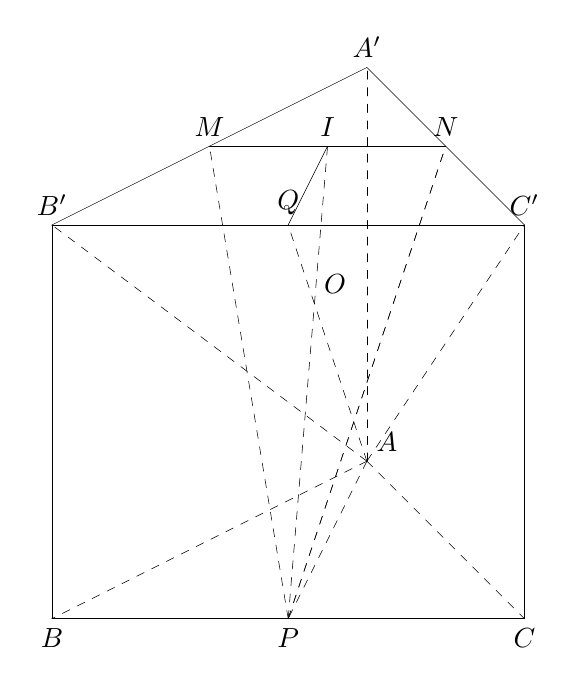
\begin{tikzpicture}[line cap=round,line join=round, >=stealth,scale=1]
			\tkzDefPoints{0/0/A, -4/-2/B, 2/-2/C, 0/5/A'}
			\coordinate (B') at ($(A')+(B)-(A)$);
			\coordinate (C') at ($(A')+(C)-(A)$);
			
			\tkzDefMidPoint(A',B') \tkzGetPoint{M}
			\tkzDefMidPoint(A',C') \tkzGetPoint{N}
			\tkzDefMidPoint(B,C) \tkzGetPoint{P}
			\tkzDefMidPoint(M,N) \tkzGetPoint{I}
			\tkzDefMidPoint(B',C') \tkzGetPoint{Q}
			\tkzInterLL(P,I)(A,Q)
			\tkzGetPoint{O}
			
			% 
			\tkzDrawSegments[dashed](A,A' A,B A,C P,M P,N A,Q P,N P,I A,B' A,C' A,P)
			\tkzDrawSegments(B,C B,B' C,C' A',B' B',C' A',C' M,N I,Q)
			\tkzLabelPoints[below](B,C,P)
			\tkzLabelPoints[above](A',B',C',Q,I,M,N)
			\tkzLabelPoints[above right](O,A)
			%\tkzLabelPoints[above left](A)
			\end{tikzpicture}
	}}
	
\end{ex}

\begin{ex}
	Trong  không  gian  Oxyz,  cho ba điểm  $A(1; 2;1), B(3; -1;1)$ và  $C(1; -1;-1)$. Gọi 
	$(S_1)$  là  mặt cầu có tâm $A$  bán kính bằng  $2$; $(S_2)$ và $(S_3)$ là hai mặt cầu có tâm lần lượt là $B,C$ và bán kính đều bằng $1$.  Hỏi có bao nhiêu mặt phẳng tiếp xúc với cả ba mặt cầu $(S_1),(S_2),(S_3)$? 
	\choice
	{$5$}
	{\True $7$}
	{$6$}
	{$8$}
	\loigiai{
		Gọi phương trình mặt phẳng $(P)$ tiếp xúc với các mặt cầu đã cho là
		$Ax+By+Cz+D =0 \,  (A^2+B^2+C^2 > 0 )$
		Tư giả thiết đề bài ta có $\mathrm{d}(A,(P)) =2, \mathrm{d}(B,(P)) =1,\mathrm{d}(C,(P)) =1$.\\
		Khi đó ta có hệ phương trình
		$\heva{& \dfrac{|A+2B+C+D|}{\sqrt{A^2+B^2+C^2}} = 2 \\ & \dfrac{|3A-B+C+D|}{\sqrt{A^2+B^2+C^2}} = 1 \\ & \dfrac{|-A-B+C+D|}{\sqrt{A^2+B^2+C^2}} = 1} \Leftrightarrow \heva{& |A+2B+C+D| = 2 \sqrt{A^2+B^2+C^2} \, (1)  \\ & |3A-B+C+D| =\sqrt{A^2+B^2+C^2}  \, (2)\\ &|-A-B+C+D| =\sqrt{A^2+B^2+C^2} \, (3)} $.\\
		Từ $(1)$ và $(2)$ , ta nhận được 
		$|3A-B+C+D| = |-A-B+C+D| \Leftrightarrow \hoac{& A = 0 \\& A-B+C+D = 0}$.\\
		Với $A = 0$, ta có: \\
		$\heva{& |2B+C+D| = 2\sqrt{B^2+C^2} \\ & |2B +C+D| = 2|-B+C+D|} \Leftrightarrow \hoac{& \heva{&  |2B+C+D| = 2\sqrt{B^2+C^2} \\ & 4B-C-D = 0 } \\ &  \heva{&  |2B+C+D| = 2\sqrt{B^2+C^2} \\ & C+D= 0 }} \Leftrightarrow
		\hoac{& \heva{&  C = \pm 2\sqrt{2}B \\ & C+D= 0 } \\ &  \heva{&  B\neq 0 \\ & 4B-C-D = 0 }} 
		$ .\\
		Do đó có ba mặt phẳng thỏa mãn.\\
		Với $A-B+C+D = 0$, ta có: \\
		$\heva{& |3B| = 2\sqrt{A^2 + B^2+C^2} \\ &  |2A| = 2\sqrt{A^2+B^2+C^2}} \Leftrightarrow \heva{&|3B|  = 4A  \\  &  |3B| = 2\sqrt{A^2+ B^2+C^2}} \Leftrightarrow  \heva{&|B|  = \dfrac{4}{3}  \\  &  |C| = \dfrac{\sqrt{11}|A|}{3} } 
		$.\\
		Do đó có bốn mặt phẳng thỏa mãn.\\
		Vậy có bảy mặt phẳng.
}
\end{ex}

\begin{ex}
	Xếp ngẫu nhiên $10$ học sinh gồm $2$ học sinh lớp $12$A, $3$ học sinh lớp $12$B và $5$ học sinh lớp $12$C thành một hàng ngang. Xác suất để trong $10$ học sinh trên không có $2$
	học sinh cùng lớp đứng cạnh nhau bằng
	\choice
	{\True $ \dfrac{11}{630}$}
	{$\dfrac{1}{126}$ }
	{$\dfrac{1}{105}$ }
	{$\dfrac{1}{42}$ }
	\loigiai{ Số phần tử của không gian mẫu là $n(\Omega) = 10!$.\\
		Gọi $A$ là biến cố "Trong $10$ học sinh không có $2$ học sinh cùng trường ngồi cạnh nhau".\\
		Xếp $5$ học sinh lớp $12C$ vào $5$ vị trí có $5!$ cách.\\
		Ứng với mỗi cách xếp $5$ học sinh lớp $12C$ sẽ có $6$ khoảng trống gồm $4$ vị trí ở giữa và $2$ vị trí hai đầu để xếp $5$ học sinh còn lại.\\
		Trường hợp $1$: Xếp $3$ học sinh lớp $12$B vào $4$ vị trí không phải vị trí hai đầu, có $\mathrm{A}_4^3$ cách.\\
		Với mỗi cách xếp trên lấy $1$ học sinh $12$A xếp vào vị trí còn lại, có $2$ cách. Do đó, học sinh còn lại có $8$ cách xếp.\\
		Số cách xếp trong trường hợp này là: $5!\mathrm{A}_4^3.2.8$ cách.\\
		Trường hợp $2$: Xếp $2$ học sinh lớp $12$B vào giữa và học sinh còn lại vào hai vị trí đầu, có $\mathrm{C_3^1}.2.\mathrm{A}_4^2$ cách.\\
		Với mỗi trường hợp trên còn $2$ vị trí trống, xếp $2$ học sinh $12A$ có $2$ cách.\\
		Số cách xếp trong trường hợp này là: $5!\mathrm{C}^1_3.2.\mathrm{A}_4^3.2$ cách.\\
		Số cách xếp là $n(A) = 5!\mathrm{C_3^1}.2.\mathrm{A}_4^2+5!\mathrm{C}^1_3.2.\mathrm{A}_4^3.2$.\\
		Vậy $P(A) = \dfrac{n(A)}{n(\Omega)} = \dfrac{11}{630}.$
	}
\end{ex}

\begin{ex}
	Cho  hàm  số $f(x)$  có đạo  hàm  liên  tục  trên đoạn 
	$[0;1]$v thỏa  mãn $f(1) =0,\, \displaystyle\int\limits_{0}^{1}[f'(x)]^2 \mathrm{\, d}x = 7$ và $\displaystyle\int\limits_{0}^{1}x^2f(x) dx \mathrm{\, d}x =\dfrac{1}{3}.$ Tích phân  $\displaystyle\int\limits_{0}^{1}f(x) \mathrm{\, d}x $ bằng
	\choice
	{\True $\dfrac{7}{5}$}
	{$1$}
	{$\dfrac{7}{4}$}
	{$4$}
	\loigiai{
		Ta có $\dfrac{1}{3} =\dfrac{1}{3} \displaystyle\int_0^1 f(x) {\mathrm d}x^3  = \dfrac{1}{3}x^3f(x)\Big|_0^1 - \dfrac{1}{3}\displaystyle\int_0^1 x^3f'(x) {\mathrm d}x  \Leftrightarrow  \displaystyle\int_0^1 x^3f'(x) {\mathrm d}x  =-1.$\\
		Mặt khác $\displaystyle\int_0^1 [f'(x)]^2 {\mathrm d}x =7 \Rightarrow \displaystyle\int_0^1\left([f'(x)]^2+14x^3f'(x)+49x^6 \right){\mathrm d}x  =0 $.\\
		Hay: 
		$\displaystyle\int_0^1\left(f'(x)+7x^3\right)^2dx = 0.$\\
		Suy ra: $ f'(x) =-7x^3.$\\
		Do đó: $ f(x) = -\dfrac{7}{4}x^4+C$. \\
		Theo đề bài $f(1) = 0 \Rightarrow f(x)=\dfrac{7}{4}(1-x^2).$\\
		Từ đó ta nhận được $I=\dfrac{7}{5}.$}
\end{ex}

\begin{ex}	
	Cho dãy số $ (u_n) $	thỏa mãn $ \log u_1 +\sqrt{2 + \log u_1 - 2 \log u_{10} } = 2 \log u_{10}$ và $ u_{n+1} = 2u_n $ với mọi $ n \ge 1. $ Giá trị nhỏ nhất của $ n $ để $ u_n > 5^{100} $ bằng
	\choice
	{$247$}
	{\True $248$}
	{$229$}
	{$290$}
	\loigiai
	{
		Ta có $ u_{n+1} = 2u_n \Rightarrow u_{10} =2^9 u_1.   $ \\ Suy ra $ \log u_1 +\sqrt{2 + \log u_1 -2 \log (2^9 u_1)} = 2 \log (2^9 u_1) $ \\
		hay $ \sqrt{2 - 18 \log 2 - \log u_1} = 18 \log 2 + \log u_1 $ \, (điều kiện $ \log u_1 > -18 \log 2 $) \\
		$ \Rightarrow \left(\log u_1\right)^2 + \left(36 \log 2 + 1\right) \cdot \log u_1 -2 +18 \log 2 = 0 \Rightarrow \hoac{&\log u_1 \simeq -4,4 \, \text{ (nhận)} \\&\log u_1 \simeq -7,5 \, \text{ (loại)}  } $\\
		Mặt khác để $ u_n > 5^{100}  \Leftrightarrow 2^{n-1} u_1 >5^{100} \Leftrightarrow n > 100 \log_2 5 - \log u_1 \cdot \log_2 10 + 1 $.\\
		Do $ n  $  là số nguyên nên giá trị nhỏ nhất của $ n  $ là 248.
	}
\end{ex}


\begin{ex}
	Có bao nhiêu giá trị nguyên của tham số $ m $ để hàm số $ y = \left|3x^4 - 4x^3 - 12x^2 + m \right| $ có 7 điểm cực trị?
	\choice
	{$ 3 $}	
	{$ 5 $}
	{\True $ 4 $}
	{$ 6 $}
	\loigiai{
		Xét $ f(x) = 3x^4 - 4x^3 - 12x^2  $.\\
		Ta có $ f'(x) =0 \Leftrightarrow  12x^3 - 12x^2 - 24x = 0 \Leftrightarrow \hoac{&x = 0  \\ &x = 2 \\&x = -1.}$
		\begin{center}
			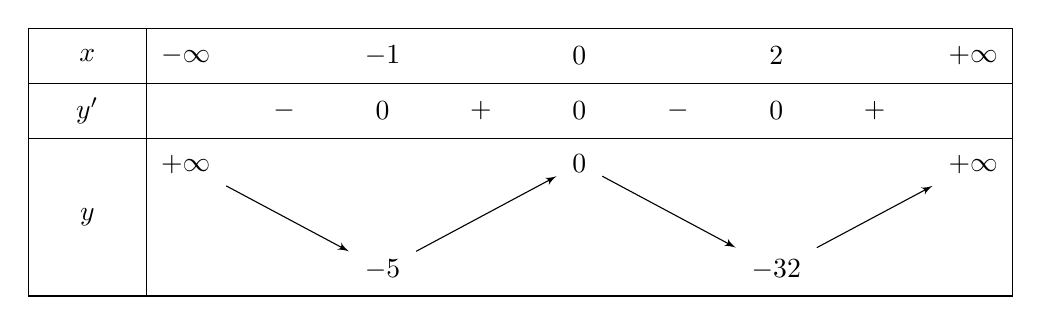
\begin{tikzpicture}
			\tkzTabInit[lgt=1.5,espcl=2.5,deltacl=.5]
			{$x$ /.7, $y’$ /.7,$y$ /2}
			{$-\infty$ , $-1$ , $0$ , $2$ , $+\infty$}
			\tkzTabLine{ ,-,$0$,+,$ 0 $,-,$ 0 $,+, }
			\tkzTabVar{+/$+\infty$ ,-/ $-5$ ,+/$0$, -/$-32$,+/$+\infty$}
			\end{tikzpicture}
		\end{center}
		Hàm số $y= \left|f(x) + m \right|  $ có 7 cực trị khi và chỉ khi $y=f(x)+m$ cắt trục hoành tại $4$ điểm phân biệt. Hay, đồ thị hàm số $y=f(x)$ cắt $y=-m$ tại $4$ điểm phân biệt.\\
		Điều này tương đương với $-5<-m<0$  hay $0<m<5$.\\
		Vậy có 4 giá trị nguyên của $ m  $ để hàm số đã cho có 7 cực trị.
	}
\end{ex}		
\begin{ex}
	Trong không gian $ Oxyz,  $	cho điểm $ A(2;2;1) $, $ B\left(-\dfrac{8}{3}; \dfrac{4}{3};\dfrac{8}{3}\right). $ Đường thẳng đi qua tâm đường tròn nội tiếp của tam giác $ OAB $ và vuông góc với mặt phẳng $ (OAB) $ có phương trình là
	\choice
	{\True $ \dfrac{x+1}{1} = \dfrac{y-3}{-2} = \dfrac{z+1}{2} $}	
	{$ \dfrac{x+1}{1} = \dfrac{y-3}{-2} = \dfrac{z-4}{2} $}
	{ $ \dfrac{x+\tfrac{1}{3}}{1} = \dfrac{y-\tfrac{5}{3}}{-2} = \dfrac{z-\tfrac{11}{6}}{2} $}
	{$ \dfrac{x+\tfrac{2}{9}}{1} = \dfrac{y-\tfrac{2}{9}}{-2} = \dfrac{z+\tfrac{5}{9}}{2} $}
	\loigiai{
		Mặt phẳng $ (OAB) $	 có véc-tơ pháp tuyến là $ \vec{n} = (1; -2;2) $ nên đường thẳng $ d $ cần tìm có VTCP $ \vec{u} = (1; -2;2)$.
		Gọi $ I $ là tâm đường tròn nội tiếp tam giác $ OAB $. \\
	Khi đó ta có $ BO \cdot \vec{IA} + OA \cdot \vec{IB} + AB \cdot \vec{IO} = \vec{0} \Rightarrow \heva{x_I = \dfrac{BO \cdot x_A + OA \cdot x_B + AB \cdot x_O}{BO + OA + AB} \\y_I = \dfrac{BO \cdot y_A + OA \cdot y_B + AB \cdot y_O}{BO + OA + AB} \\ z_I = \dfrac{BO \cdot z_A + OA \cdot z_B + AB \cdot z_O}{BO + OA + AB}}  \Rightarrow I(0;1;1).$\\
	Vậy phương trình đường thẳng cần tìm $ \dfrac{x+1}{1} = \dfrac{y-3}{-2} = \dfrac{z+1}{2} $.
}
\end{ex}		
\begin{ex}
	Cho hai hình vuông $ ABCD $	và $ ABEF $ có cạnh bằng $ 1 $, lần lượt nằm trên hai mặt phẳng vuông góc với nhau. Gọi $ S $ là điểm đối xứng với $ B $ qua đường thẳng $ DE $. Tính thể tích của khối da diện $ ABCDSEF $.
	\choice
	{$ \dfrac{7}{6} $}	
	{$ \dfrac{11}{12} $}
	{$ \dfrac{2}{3} $}
	{\True $ \dfrac{5}{6} $}
	\loigiai
	{Chọn hệ trục tọa độ sao cho hình vuông $ ABCD $ trên mp$ (Oxy)$, hình vuông $ ABEF $ nằm trên mặt phẳng $ (Oxz) $ và $ A $ trùng gốc tọa độ. Khi đó $ A(0;0;0), B(1;0;0), D(0;1;0), F(0;0;1) $	suy ra $ E(1;0;1). $
		\begin{center}
		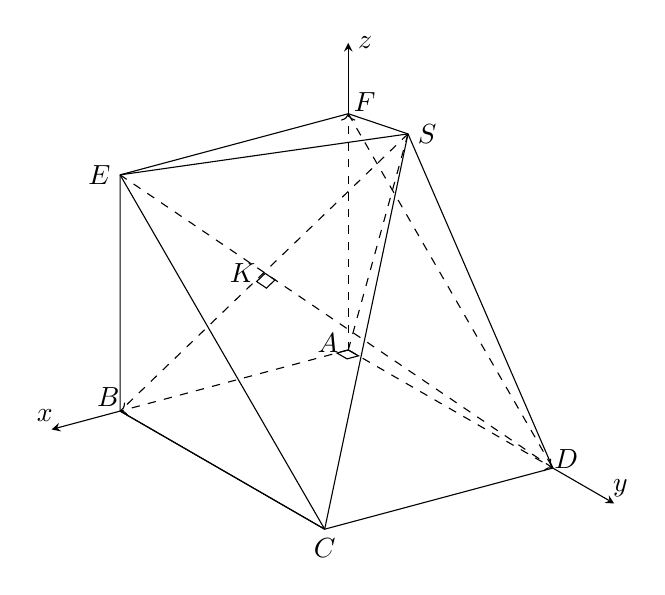
\begin{tikzpicture}
		[x={({sin(-75)*1cm},{-cos(75)*1cm})},y={(0.866cm,-0.5cm)},z={(0cm,1cm)},scale = 3]
		\coordinate (a) at (0,0,0);
		\coordinate (d) at (0,1,0);
		\coordinate (b) at (1,0,0);
		\coordinate (k) at (0.66,0.33,0.66);
		\draw [->,dashed] (0,0,0)--(1,0,0) ;
		\draw [->,dashed] (0,0,0)--(0,1,0) ;
		\draw [->,dashed] (0,0,0)--(0,0,1) ;
				\draw [>=stealth] (1,0,0)--(1,1,0);
				\draw [>=stealth] (1,0,0)--(1,1,0)--(0,1,0)--(0.33,0.66,1.33)--(1,0,1)--(1,0,0);
				\draw [>=stealth] (0.33,0.66,1.33)--(0,0,1)--(1,0,1);
				\draw [>=stealth] (0.33,0.66,1.33)--(1,1,0);
		\draw [dashed] (0.33,0.66,1.33)--(1,0,0);
		\draw [dashed] (0.33,0.66,1.33)--(0,0,0);
		\draw [dashed] (0,1,0)--(1,0,1);
		\draw (1,0,1)--(1,1,0);
		\node at (0,0,0.03) [left] {$ A $};
		\node at (0.96,0,0.05) [left] {$ B $};
		\node at (0,0.96,0.02) [right] {$ D $};
		\node at (0,-0.02,1.04) [right] {$ F $};
		\node at (1,0,1) [left] {$ E $};
		\node at (1,1,0) [right, below] {$ C $};
		\draw[>=stealth,->] (1,0,0)--(1.3,0,0) node [pos = 1.1][above] {$ x $};
		\draw [>=stealth,->] (0,1,0)--(0,1.3,0) node [pos = 1.1] [above]{$ y $};
		\draw[>=stealth,->] (0,0,1)--(0,0,1.3) node [pos = 1] [right]{$ z $};
		\draw [>=stealth,dashed] (0,0,1)--(0,1,0);
		\node at (0.66,0.33,0.66) [left] {$ K $};
		\node at (0.33,0.66,1.33) [right] {$ S $};
		\tkzMarkRightAngle[size=0.05](d,k,b);
		\tkzMarkRightAngle[size=0.05](d,a,b);
			\end{tikzpicture}
		\end{center} 
		Phương trình đường thẳng $ DE: \heva{&x = t \\&y = 1-t\\&z = t. } $\\
		Mặt phẳng $ (P) $ qua $ B $ và vuông góc $ DE $ cắt $ DE $ tại $ K $ có phương trình $ x - y + z - 1 = 0$.\\
		$ \Rightarrow K = DE \cap (P) $  có tọa độ là $ K = \left(\dfrac{2}{3}; \dfrac{1}{3}; \dfrac{2}{3}\right) $.\\
		Do $ S $ là điểm đối xứng của $ B $ qua $ DE $ nên $ S =  \left(\dfrac{1}{3}; \dfrac{2}{3}; \dfrac{4}{3}\right) $.
		\begin{itemize}
			\item 		Cách 1: $ V = V_{SABCD} + V_{SABEF} + V_{SADF}+V_{SBCE}= \dfrac{1}{3} \cdot \dfrac{4}{3} + \dfrac{1}{3} \cdot \dfrac{2}{3} + \dfrac{1}{3} \cdot \dfrac{1}{2} \cdot \dfrac{1}{3} + \dfrac{1}{3} \cdot \dfrac{1}{2} \cdot \dfrac{2}{3} = \dfrac{5}{6} $.
			\item Cách 2: Thể tích khối đa diện $ ABCDSEF  $ là $ V_{ABCDSEF} = V_{SCDFE} + V_{ABCDEF}.$\\
			Trong đó: 
			$V_{SCDFE} = \dfrac{1}{3} d\left(S,(CDFE)\right) \cdot S_{CDFE} = \dfrac{1}{3} \cdot \dfrac{1}{\sqrt{2}} \cdot \sqrt{2} = \dfrac{1}{3} $ và $ V_{ABCDEF} = \dfrac{1}{2} $.
		\end{itemize}
		Vậy thể tích cần tìm là $ V = \dfrac{1}{3} + \dfrac{1}{2} = \dfrac{5}{6}.$ 
	}
\end{ex}	
\Closesolutionfile{ans}
\section{Các cách in đáp án trắc nghiệm}
Cấu trúc lệnh
\begin{verbatim}
\inputans{số cột}{đường dẫn lưu file ans}%theo hàng ngang
\inputansbox{số cột}{đường dẫn lưu file ans}%dạng hộp/bảng
\end{verbatim}
\begin{center}
\textbf{ĐÁP SỐ CÂU HỎI TRẮC NGHIỆM (theo hàng ngang 10 cột)}
\end{center}
\inputans{10}{ans/anstest}
\begin{center}
\textbf{ĐÁP SỐ CÂU HỎI TRẮC NGHIỆM (theo hàng ngang 5 cột)}
\end{center}
\inputans{5}{ans/anstest}
\begin{center}
\textbf{ĐÁP SỐ CÂU HỎI TRẮC NGHIỆM (dạng hộp/bảng 10 cột)}
\end{center}
\inputansbox{10}{ans/anstest}
\begin{center}
\textbf{ĐÁP SỐ CÂU HỎI TRẮC NGHIỆM (dạng hộp/bảng 5 cột)}
\end{center}
\inputansbox{5}{ans/anstest}

\end{document}
